% -*- mode:flyspell; mode:latex -*-
\documentclass[12pt]{article}
\addtolength{\oddsidemargin} {-0.885in}
\addtolength{\textwidth}{1.75in}
\addtolength{\evensidemargin}{-0.8in}


\usepackage[latin1]{inputenc}
\usepackage[T1]{fontenc}
\usepackage[english]{babel}
\usepackage{graphicx}
\usepackage{float}
%% \usepackage{siunitx}

%% \usepackage{gensymb}


\usepackage{tikz}
\usepackage{[caption}
\usetikzlibrary{arrows}
\usetikzlibrary{decorations.markings}
\usetikzlibrary{decorations.pathmorphing}
% \usepackage[absolute,overlay]{textpos}
% \usepackage{onimage}

\usepackage{tabularx}
\usepackage{times}
\usepackage{graphics}

% \usepackage{subfigure}
% \usepackage{scalefnt}
%
% \renewcommand\thesubfigure{\arabic{subfigure}}

\usepackage{amsmath}
\usepackage{hyperref}
\usepackage{hhline}
\usepackage{subfig}
\usepackage{color}
\usepackage[all]{hypcap}

\usepackage[normalem]{ulem}  % for striking out
\usepackage{soul}
% \usepackage{fancyhdr}
% \pagestyle{fancy}
% \fancyhead[C]{}
% \fancyhead[L] {\it{Mu2e-doc-29670-v1.0} }
%%%%%%%%%%%%%%%%%%%%%%%%%%%%%%%%%%%%%%%%%%%%%%%%%%%%%%%%%%%%%%%%%%%%%%%%%%%%%%
% use natbib - biblatex not available on Mu2e interactive nodes
%%%%%%%%%%%%%%%%%%%%%%%%%%%%%%%%%%%%%%%%%%%%%%%%%%%%%%%%%%%%%%%%%%%%%%%%%%%%%%
\usepackage[square,sort,comma,numbers]{natbib}

% location of the .bib files: env var BIBINPUTS (~/library/bibliography)

% \usepackage[backend=biber, style=numeric-comp, sorting=ynt] {biblatex}
% \addbibresource{clfv.bib}

% \addbibresource{stntuple.bib}
% \addbibresource{mu2e_web.bib}
% \addbibresource{radiative_pion_capture.bib}

\graphicspath{{figures/}}
%%%%%%%%%%%%%%%%%%%%%%%%%%%%%%%%%%%%%%%%%%%%%%%%%%%%%%%%%%%%%%%%%%%%%%%%%%%%%%
% for portability, make sure all commands are included locally,
%%%%%%%%%%%%%%%%%%%%%%%%%%%%%%%%%%%%%%%%%%%%%%%%%%%%%%%%%%%%%%%%%%%%%%%%%%%%%%
\definecolor{ForestGreen}{RGB}{20,109,20}
%\include{commands}
\newcommand {\blue}      {\color{blue}}
\newcommand {\green}     {\color{ForestGreen}}
\newcommand {\red}       {\color{red}}
\newcommand {\purple}    {\color{purple}}
\newcommand {\violet}    {\color{violet}}

\newcommand {\kmax}      {\mbox{$k_{\rm max}$}}
\newcommand {\piplusenu} {\mbox{$\pi^+ \to e^+ \nu$}}

\newcommand {\mumemconv}[1][A] {\mbox{$\mu^- \textrm{#1} \rightarrow e^- \textrm{#1}$}}
% Define a relay to have 2 default arguments instead of limit of 1
\newcommand {\mumepconv}[1][A] {%
  \def\ArgI{{#1}}%store the first argument
  \mumepconvRelay
}
\newcommand \mumepconvRelay[1][A]  {\mbox{$\mu^- \textrm{\ArgI} \rightarrow e^+ \textrm{#1}$}}
\newcommand {\MuToEm}     {\mbox{$\mu^- \ra e^-$}}
\newcommand {\MuToEp}     {\mbox{$\mu^- \ra e^+$}}
\newcommand {\MuPToEp}    {\mbox{$\mu^+ \ra e^+$}}
\newcommand {\ra}        {\rightarrow}
\newcommand {\Rmue}       {\mbox{$R_{\mu e}$}}
\newcommand {\tandip}    {\mbox{$\tan \lambda$}}

\newcommand {\Pb}[1]     {\mbox{$\rm ^{#1}Pb$}}                 % isotopes of lead
\newcommand {\Au}[1]     {\mbox{$\rm ^{#1}Au$}}                 % isotopes of gold
\newcommand {\Ir}[1]     {\mbox{$\rm ^{#1}Ir$}}                 % isotopes of iridium
%%%%%%%%%%%%%%%%%%%%%%%%%%%%%%%%%%%%%%%%%%%%%%%%%%%%%%%%%%%%%%%%%%%%%%%%%%%%%%
% editing commands
%%%%%%%%%%%%%%%%%%%%%%%%%%%%%%%%%%%%%%%%%%%%%%%%%%%%%%%%%%%%%%%%%%%%%%%%%%%%%%
\newcommand {\del}[1]    {{\blue   \sout{#1}}}
\newcommand {\dlt}[1]    {{\violet \sout{#1}}} %alternate delete color
\newcommand {\add}[1]    {{\red #1}}
\newcommand {\alt}[1]    {{\green #1}} %alternate comment color
\newcommand {\hlite}[1]  {{\red      \ul{#1}}}   % needs xcolor, soul
% %%%%%%%%%%%%%%%%%%%%%%%%%%%%%%%%%%%%%%%%%%%%%%%%%%%%%%%%%%%%%%%%%%%%%%%%%%%%%%
% for editors
% %%%%%%%%%%%%%%%%%%%%%%%%%%%%%%%%%%%%%%%%%%%%%%%%%%%%%%%%%%%%%%%%%%%%%%%%%%%%%%
\newcommand {\pasha}[1]    {{\green  #1}}
\newcommand {\kate}[1]     {{\blue   #1}}
%%%%%%%%%%%%%%%%%%%%%%%%%%%%%%%%%%%%%%%%%%%%%%%%%%%%%%%%%%%%%%%%%%%%%%%%%%%%%%
\begin{document}

\begin{titlepage}
  \begin{flushright}
    \bf {MU2E/PHYSICS/50071} \\
    version 1.01
    \today
 \end{flushright}

  \vspace{1cm}

  \begin{center}
    {\Large \bf On a possibility of the Mu2e momentum scale calibration at full field
      \vspace{0.3in}
      1. Proof of principle
    }

    \vspace{1cm}
    K.Ciampa, J.Miller(BU), P.Murat(FNAL)

    % \footnote{\texttt{Fermilab; e-mail: murat@fnal.gov}}
    \vspace{0.3cm}

    \vspace{0.8cm}
  \end{center}

  \begin{abstract}
    \vspace{0.2in}
    
    The pion degrader reduces the background from muon decays in flight to facilitate
    the momentum scale calibration with \piplusenu\ decays. That calibration needs to
    be performed at $B \simeq 0.7$ T, so the determined momentum scale would need to be
    extrapolated to the nominal field value, B = 1 T.
    
    With small modifications, the pion degrader could become an instrument
    also allowing to calibrate the Mu2e momentum scale in full field.
    The calibration at full field is based on reconstruction of a 129.4 MeV photon
    peak from RPC on hydrogen, $\pi^- p \to n \gamma$.
%
    The converted photon energy is given by the $e^+e^-$ invariant mass,
    This note demonstrates that due to relatively small multiple scattering,
    the sum of the electron an positron momenta gives a good approximation
    of the $e^+e^-$ invariant mass. Thus reconstruction of the energy of a photon
    converted several meters in upstream of the tracker only needs the $e^+$ and $e^-$
    track momenta to be reconstructed, but doesn't require the track extrapolation
    back to the degrader.

    Under realistic assumptions, the time needed to calibrate the momentum scale
    to the accuracy better then 100 keV while running at 10\% of the nominal proton beam
    intensity is about one day.

  \end{abstract}

\end{titlepage}
% \frontmatter
% \chapter*{Abstract}
%
% \addcontentsline{toc}{chapter}{Abstract}
%
% \mainmatter
%
{\tableofcontents}

%%%%%%%%%%%%%%%%%%%%%%%%%%%%%%%%%%%%%%%%%%%%%%%%%%%%%%%%%%%%%%%%%%%%%%%%%%%%%%%
%\chapter{Calibration}
%%%%%%%%%%%%%%%%%%%%%%%%%%%%%%%%%%%%%%%%%%%%%%%%%%%%%%%%%%%%%%%%%%%%%%%%%%%%%%%
% \input{input_data}

%%%%%%%%%%%%%%%%%%%%%%%%%%%%%%%%%%%%%%%%%%%%%%%%%%%%%%%%%%%%%%%%%%%%%%%%%%%%%%%

\newpage
\section {Revision History and TODO items}

\begin{itemize}
\item
  v1.01: inital version
\end{itemize}

{\red
TODO items:

\begin{itemize}
\item
  check references
\item
  check section names
\item
  add scripted fits with printed fit errors with enough digits 
\item
  describe datasets
\end{itemize}
}
%%%%%%%%%%%%%%%%%%%%%%%%%%%%%%%%%%%%%%%%%%%%%%%%%%%%%%%%%%%%%%%%%%%%%%%%%%%%%%
\newpage
\section {Introduction}
Negative pions stopped in hydrogen get captured by the hydrogen atoms, 
with the following interactions proceeding via two main channels:
$\pi^- p \to n\pi^0$ and $\pi^- p \to n \gamma$.

The second channel has a branching ratio close to 40\% and as both initial state particles
are at rest, the outgoing photons are monochromatic with the energy E=129.4 MeV~\cite{something_on_RPC}.

The 129.4 MeV peak from $\pi^- p \to n \gamma$ is also clearly visible on hydrogen-containing
compounds, for example, polyethylene \cite{}.

Using such a compound as a material for the Mu2e pion degrader disk may allow to calibrate
the Mu2e momentum scale at B = 1 T.

The scale calibration requires one additional element - a this converter ring located next
to the degrader at a sufficiently large radius, of the order of R $\sim$ 25 cm.
Photons converted there would produce a $e^+e^-$ pair, with both an electron and
a positron producing sufficient number of the tracker hits for both tracks
to be reconstructed. The converted photon energy can be then determined as the sum
of the two reconstructed track momenta, $E = P_{e^-} + P_{e^+}$ 
All momentum scale calibration approaches discussed so far assume that the magnetic field
in the detector solenoid is reduced \cite{MU2E_48630_PIPLUSENU}.
An advantage of the calibration discussed in this note is that it can be performed
without reducing the DS magnetic field.


%%%%%%%%%%%%%%%%%%%%%%%%%%%%%%%%%%%%%%%%%%%%%%%%%%%%%%%%%%%%%%%%%%%%%%%%%%%%%%
\section{RPC on hydrogen}

Has been measured in \cite{RPC_1972_Bistirlich_PhysRevC.5.1867}.

Events of interest for calibration are the monochomatic RPC photons at 129.4 MeV from $\pi^{-} p \to n \gamma$ on
hydrogen. Measurement of this process is shown in 
Figure~\ref{figure:1971_bistirlich_fig_02_h2}
, the photon energy spectrum from pion capture on hydrogen, which also includes lower energy photons from the charge exchange reaction. 
For the $\rm{CH_2}$ spectrum in 
Figure~\ref{figure:1971_bistirlich_fig_09_ch2}
, photons from RPC on carbon occupy the region between the two hydrogen peaks.
To produce a photon in the 129.4 MeV peak, a negative pion stopped on
a $\rm{CH_2}$  degrader must both (i) capture on a hydrogen rather than carbon nucleus, and (ii) interact
radiatively with the proton via $\pi^{-} p \to n \gamma$ rather than producing an intermediate $\pi^0$.


\begin{figure}[H]
 \begin{minipage}{.5\textwidth}
  \includegraphics[width=0.9\textwidth]{png/1971_bistirlich_fig_02_h2}
  \captionsetup{width=.8\linewidth}
  \caption[width=0.9\textwidth]{
      \label{figure:1971_bistirlich_fig_02_h2}
    \kate{Photon energy spectrum from negative pion capture on hydrogen \cite{RPC_1972_Bistirlich_PhysRevC.5.1867}.}
    }
 \end{minipage}
 \begin{minipage}{.5\textwidth}
  \includegraphics[width=0.9\textwidth]{png/1971_bistirlich_fig_09_ch2}
  \captionsetup{width=.8\linewidth}
  \caption[width=0.9\textwidth]{
  \label{figure:1971_bistirlich_fig_09_ch2}
    \kate{Photon energy spectrum from negative pion capture on $\rm{CH_2}$ \cite{RPC_1972_Bistirlich_PhysRevC.5.1867}.}
   }
 \end{minipage}
\end{figure}

The probability of pion capture on the hydrogen component of the $\rm{CH_2}$ compound is
$\rm{ W_H = (12.9 \pm 1.8) \times 10^{-3 }}$
 as used in Ref.~X \path{1991_Harston_PhysRevA.44.103}
 , an average of previous measurements. 
 This accounts for both hydrogen atoms in the $\rm{CH_2}$ molecule, and is larger than but consistent with the
 corresponding measurement (expressed as percent) in Ref.~\cite{RPC_1972_Bistirlich_PhysRevC.5.1867}.
 Negative pions captured on hydrogen have a $ (41.4 \pm 3.2) \% $
 probability of interacting via $\pi^{-} p \to n \gamma$ and producing a photon at 129.4 MeV
 \cite{RPC_1972_Bistirlich_PhysRevC.5.1867}.
 The remaining pions captured on hydrogen produce two photons via the charge exchange reaction
 $ \pi^{-} p \to n \pi^0 $ with $\pi^0  \to \gamma \gamma $,
 which results in the lower energy peak of the hydrogen spectrum. 

Together these factors yield a probability of $ (5.34 \pm 0.85) \times 10^{-3} $
for obtaining 129.4 MeV RPC photons from pion capture on $\rm{CH_2}$.

% \bigskip
%  Additional reference for \path{radiative_pion_capture.bib}:
% {\tiny
% {\begin{verbatim}
% @article{1991_Harston_PhysRevA.44.103,
%   title = {Capture and transfer of stopped pions in alcohols},
%   author = {Harston, M. R. and Armstrong, D. S. and Measday, D. F. and Stanislaus, S. and Weber, P. and Horv\'ath, D.},
%   journal = {Phys. Rev. A},
%   volume = {44},
%   issue = {1},
%   pages = {103--110},
%   numpages = {0},
%   year = {1991},
%   month = {Jul},
%   publisher = {American Physical Society},
%   doi = {10.1103/PhysRevA.44.103},
%   url = {https://link.aps.org/doi/10.1103/PhysRevA.44.103}
% }
% \end{verbatim}}}
% 

\kate{
\bigskip
  Potential changes:
  \begin{itemize}
  \item 
    Include individual previous measurements if needed.
  \end{itemize}
}


%%% Local Variables:
%%% mode: latex
%%% TeX-master: t
%%% End:

%%%%%%%%%%%%%%%%%%%%%%%%%%%%%%%%%%%%%%%%%%%%%%%%%%%%%%%%%%%%%%%%%%%%%%%%%%%%%%
\section{Degrader geometry}

The pion degrader was initially introduced in order to suppress the background to \piplusenu\
from muon decays in flight. The degrader is a movable disk made of non-magnetic material,
which gets inserted into the beam during the calibration runs and moved out of the beam
during the regular data taking.

\begin{figure}[H]
  \begin{tikzpicture}
    \node[anchor=south west,inner sep=0] at (0,-10.) {
      % \node[shift={(0 cm,0.cm)},inner sep=0,rotate={90}] at (0,0) {}
      \makebox[\textwidth][c] {
        \includegraphics[width=0.95\textwidth]{pdf/degrader_geometry_002}
      }
    };
    % \node [text width=8cm, scale=1.0] at (14.5,0.5) {$\mu_B$, expected background mean};
    % \node [text width=8cm, scale=1.0, rotate={90}] at (1.5,7.5) { $S_{D}$, ``discovery'' signal strength  };
  \end{tikzpicture}
  \caption{
    \label{figure:degrader_geometry_001}
    Schematic view of the simulated degrader geometry, not up to scale
  }
\end{figure}

The simulated degrader geometry is schematically shown in Figure~\ref{figure:degrader_geometry_001}.
A gold converter ring has the outer radius $R_{out}$ = 250mm, and the value of $R_{in}$ is defined
by the converter thickness. The converter is slightly offset downstream wit respect to the $CH_2$ disk,
so $e*+$ and $e^-$ produced in the converter do not cross it multiple times.

\begin{itemize}
\item 
  From \piplusenu\ studies: the pion degrader disk thickness of 4 mm Ti is close to optimal.
\item
  4mm of Ti translates into the total amount of material of $\sim 1.8 g/cm^2$,
  about twice the material of the stopping target.
\item
  9mm CH2 + 1.0mm Pb: : 2.0 $g/cm^2$   .. $\pi*15^2*(0.9*0.95 + 0.08*11.34): \simeq 2 g/cm^2$
\item
   9mm CH2 + 0.8mm Pb: : $1.76 g/cm^2$
 \item
   CH2 disk R=14 cm, weight        : $0.90*0.95*\pi*14^2 ~= 526$ gr \\
   Pb  foil R=10cm thickness 0.8mm : $0.08*11.34*\pi*10^2 = 285$ gr \\
   total                           : 811 gr
\end{itemize}

To make sure that $e^+$ and $e^-$ do not cross the converter foil multiple times,
the converter is moved downstream by 1cm with respect to the degrader disk.

The converter foil could be supported by a carbon foam disk surrounding the degrader.
A potentially more attractive alternative could be to have the converter placed
on a thin carbon foam ring and supported from the OPA. 
As the $\gamma \to e^+e^-$ acceptance is proportional to the width of the converter ring,
making it, for example, 3cm wide instead of 1 cm wide would increase the acceptance
by a factor close to x3.

This option is discussed in Section~\ref{section:geometry_v4}


%%%%%%%%%%%%%%%%%%%%%%%%%%%%%%%%%%%%%%%%%%%%%%%%%%%%%%%%%%%%%%%%%%%%%%%%%%%%%%
\subsection{Stopped negative pions}

\begin{itemize}
\item 
  Simulation of the negative pion beam follows the standard 2-stage model.
  Stage 2 produces three separate datasets of pions stops in the CH2, Pb, and the ST.
  The scheme allow to resimulate the pion stop datasets w/o repeating more time consuming
  first stage of the simulation.
\item
  To improve the simulation efficiency pion decays are disabled. The calculated by Geant4
  pion survival probabilities are used as event weights in the normalization procedure.
\end{itemize}

Distributions of momentum and time for pions stopped in it CH2, Pb foil, and the
stopping target are shown in Figure \ref{figure:stopped_pim_mom_time}.

\begin{figure}[H]
  \begin{tikzpicture}
    \node[anchor=south west,inner sep=0] at (0,0.) {
      % \node[shift={(0 cm,0.cm)},inner sep=0,rotate={90}] at (0,0) {}
      % \makebox[\textwidth][c] {
        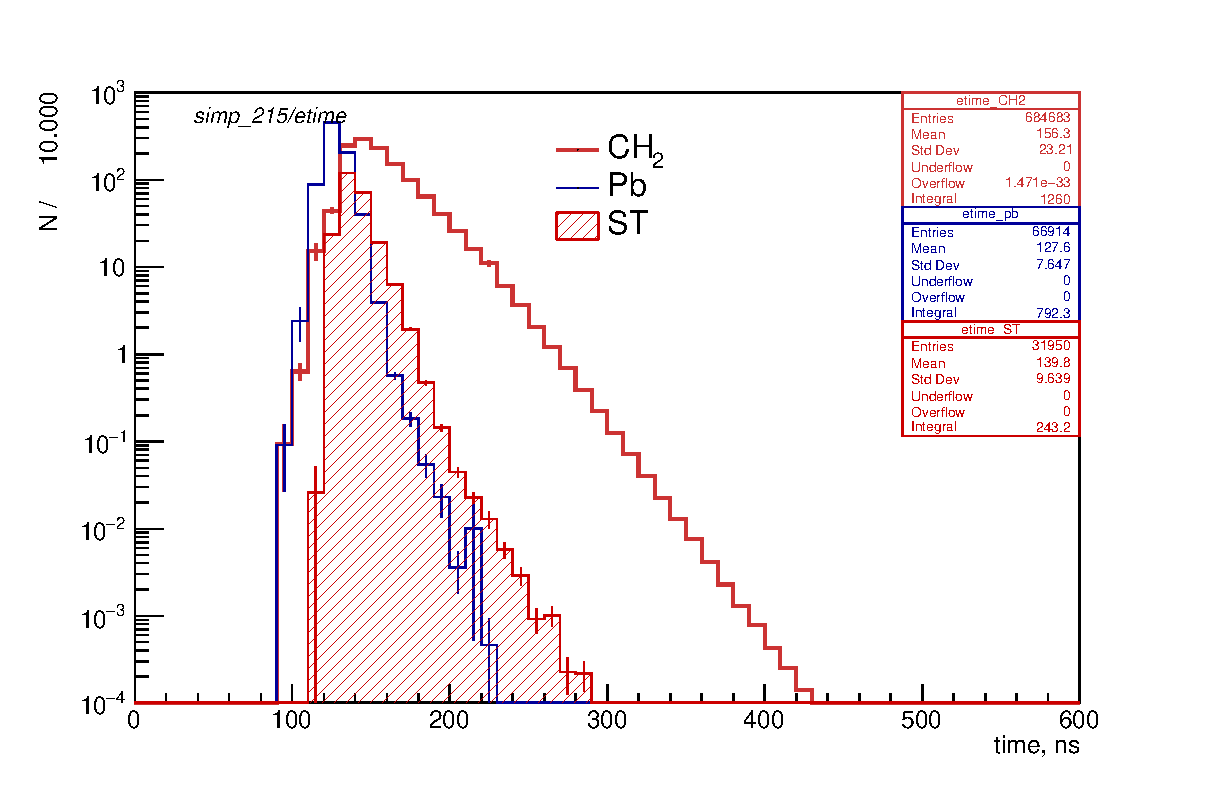
\includegraphics[width=0.5\textwidth]{pdf/figure_00021}
      % }
    };
    \node[anchor=south west,inner sep=0] at (10,0.) {
      % \node[shift={(0 cm,0.cm)},inner sep=0,rotate={90}] at (0,0) {}
      % \makebox[\textwidth][c] {
        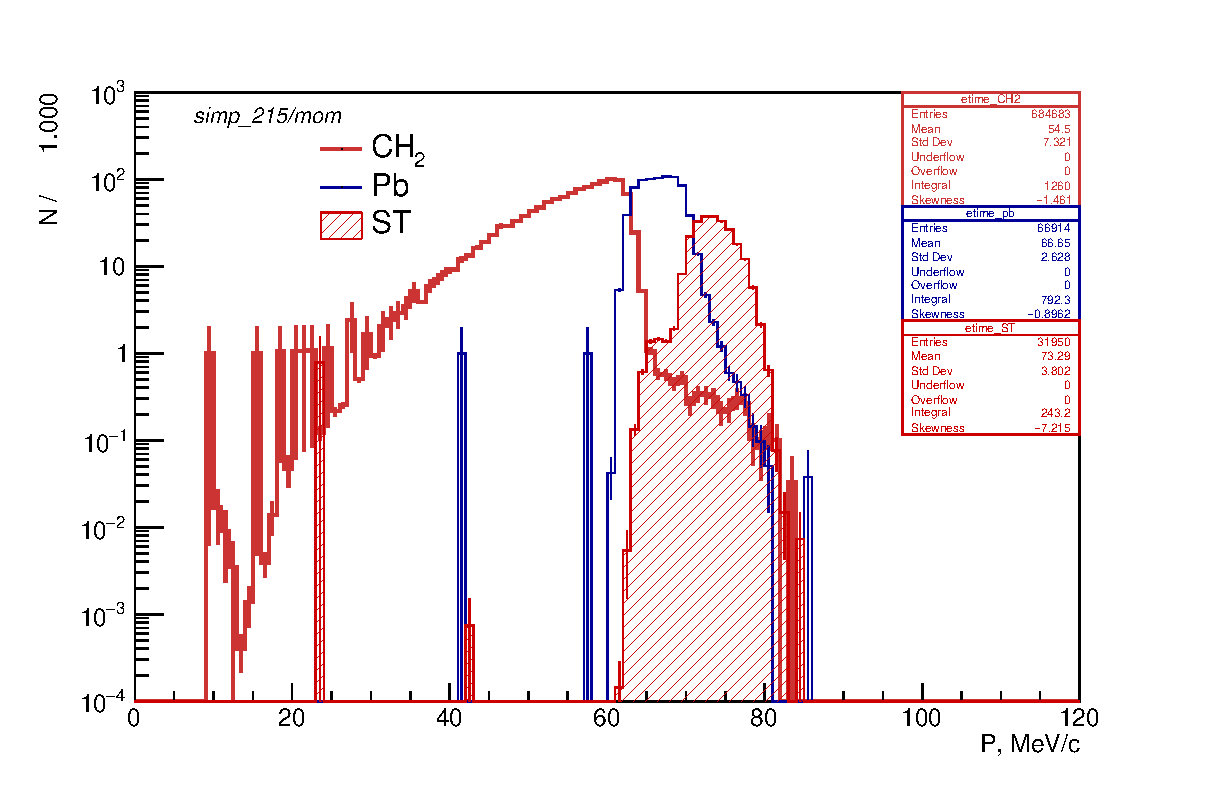
\includegraphics[width=0.5\textwidth]{pdf/figure_00022}
      % }
    };
    % \node [text width=8cm, scale=1.0] at (14.5,0.5) {$\mu_B$, expected background mean};
    % \node [text width=8cm, scale=1.0, rotate={90}] at (1.5,7.5) { $S_{D}$, ``discovery'' signal strength  };
  \end{tikzpicture}
  \caption{
    \label{figure:stopped_pim_mom_time}
    Stopped pions: distributions of momentum and time
  }
\end{figure}

It is worth noting that pions stopped in the $CH_2$ are the slowest ones.
Therefore, selecting events with the pion stop time above certain threshold, i.e. $\sim 200$ ns, 
significantly suppresses contributions of the stopping target and the Pb foil to any measurement.
T0 = 200 ns is also approximately the time where the instantaneous beam flash
hit rate gets reduced down to the level allowing the measurements. For the DAQ operations,
that means that the digitization start time should be lowered to $\sim 250$ ns,
which, at a reduced proton beam intensity, looks quite realistic.

Another interesting correlation is the correlation between the pion momentum on exit from the TS momentum
and the vertical coordinate of the pion stop point. Figure ~\ref{figure:y_vs_p_deg} shows this correlation
for pions stopped in the $CH_2$ and Pb parts of the degrader. The Y distribution of the pion stops
in the Pb foil is offset down by several centimeters. The lower cut-off at R=100 mm is determined by the
by the simulated radius of the Pb foil, R=100mm

\begin{figure}[H]
  \begin{tikzpicture}
    \node[anchor=south west,inner sep=0] at (0,0.) {
      % \node[shift={(0 cm,0.cm)},inner sep=0,rotate={90}] at (0,0) {}
      %\makebox[\textwidth][c] {
        \includegraphics[width=0.5\textwidth]{png/figure_00036}
      %}
    };
    \node[anchor=south west,inner sep=0] at (10.,0.) {
      % \node[shift={(0 cm,0.cm)},inner sep=0,rotate={90}] at (0,0) {}
      % \makebox[\textwidth][c] {
      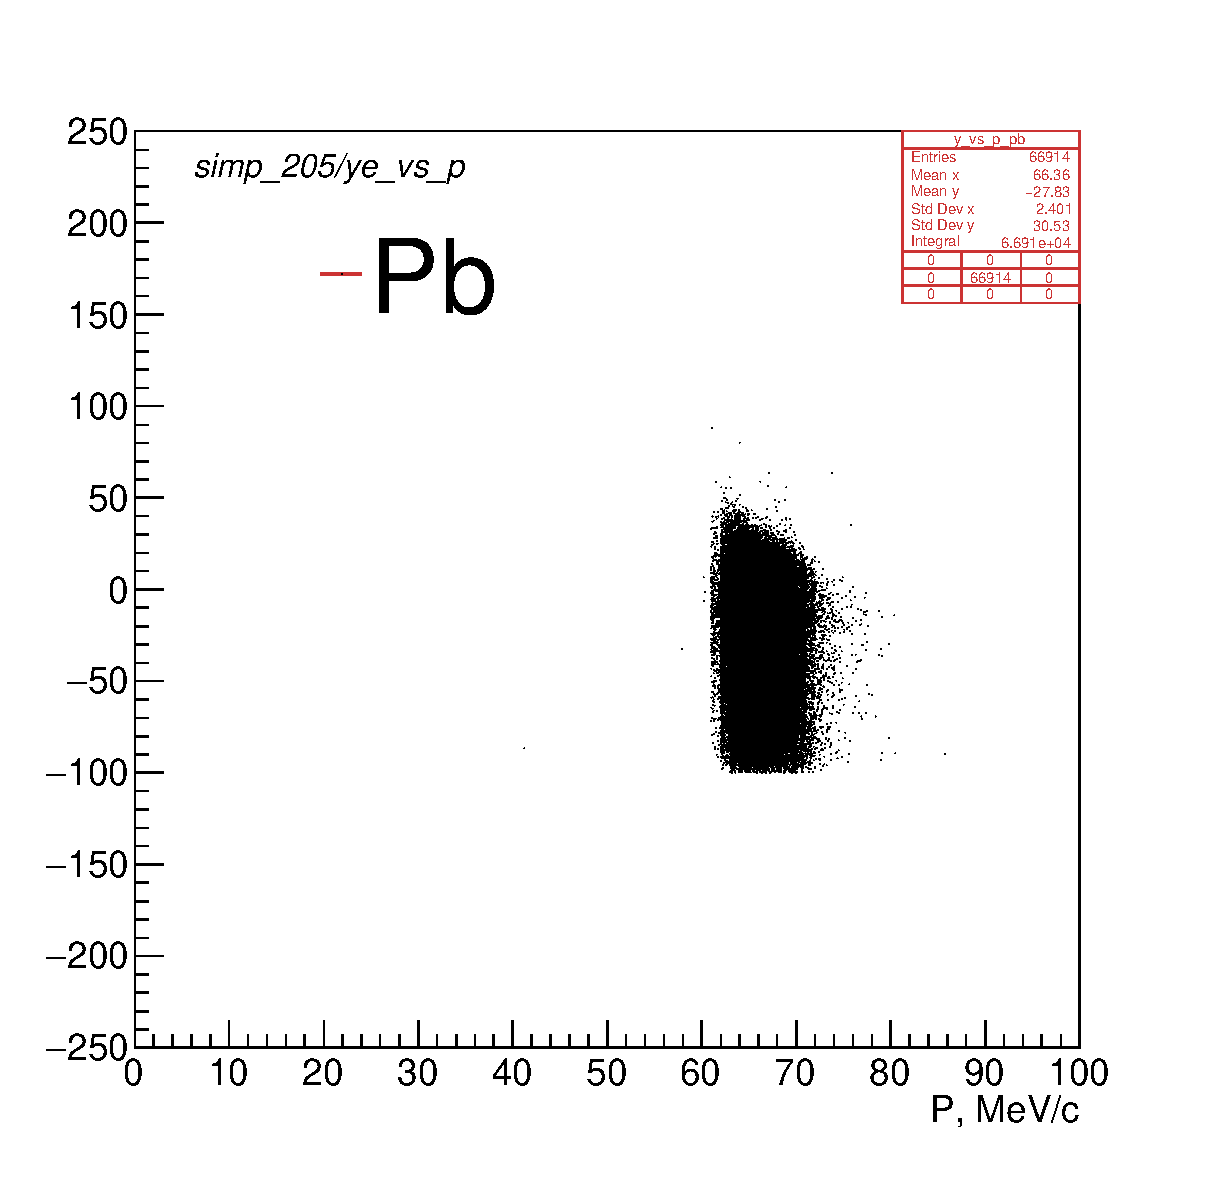
\includegraphics[width=0.5\textwidth]{png/figure_00037}
      %} 
    };
    % \node [text width=8cm, scale=1.0] at (14.5,0.5) {$\mu_B$, expected background mean};
    % \node [text width=8cm, scale=1.0, rotate={90}] at (1.5,7.5) { $S_{D}$, ``discovery'' signal strength  };
  \end{tikzpicture}
  \caption{
    \label{figure:y_vs_p_deg}
    Y(stop):P\@(DS entrance) for negative pions stopped in the $CH_2$ and Pb parts of the simulated degrader
  }
\end{figure}

Y:X distributions of the pion stops in the $CH_2$ disk, Pb foil and the ST are shown in Figure ~\ref{figure:y_vs_x_st}.
They reflect the correlation between the mean Y of the particle trajectory and the particle momentum.

\begin{figure}[H]
  \begin{tikzpicture}
    \node[anchor=south west,inner sep=0] at (0,0.) {
      % \node[shift={(0 cm,0.cm)},inner sep=0,rotate={90}] at (0,0) {}
      %\makebox[\textwidth][c] {
        \includegraphics[width=0.5\textwidth]{png/figure_00034}
      %}
    };
    \node[anchor=south west,inner sep=0] at (10.,0.) {
      % \node[shift={(0 cm,0.cm)},inner sep=0,rotate={90}] at (0,0) {}
      %\makebox[\textwidth][c] {
        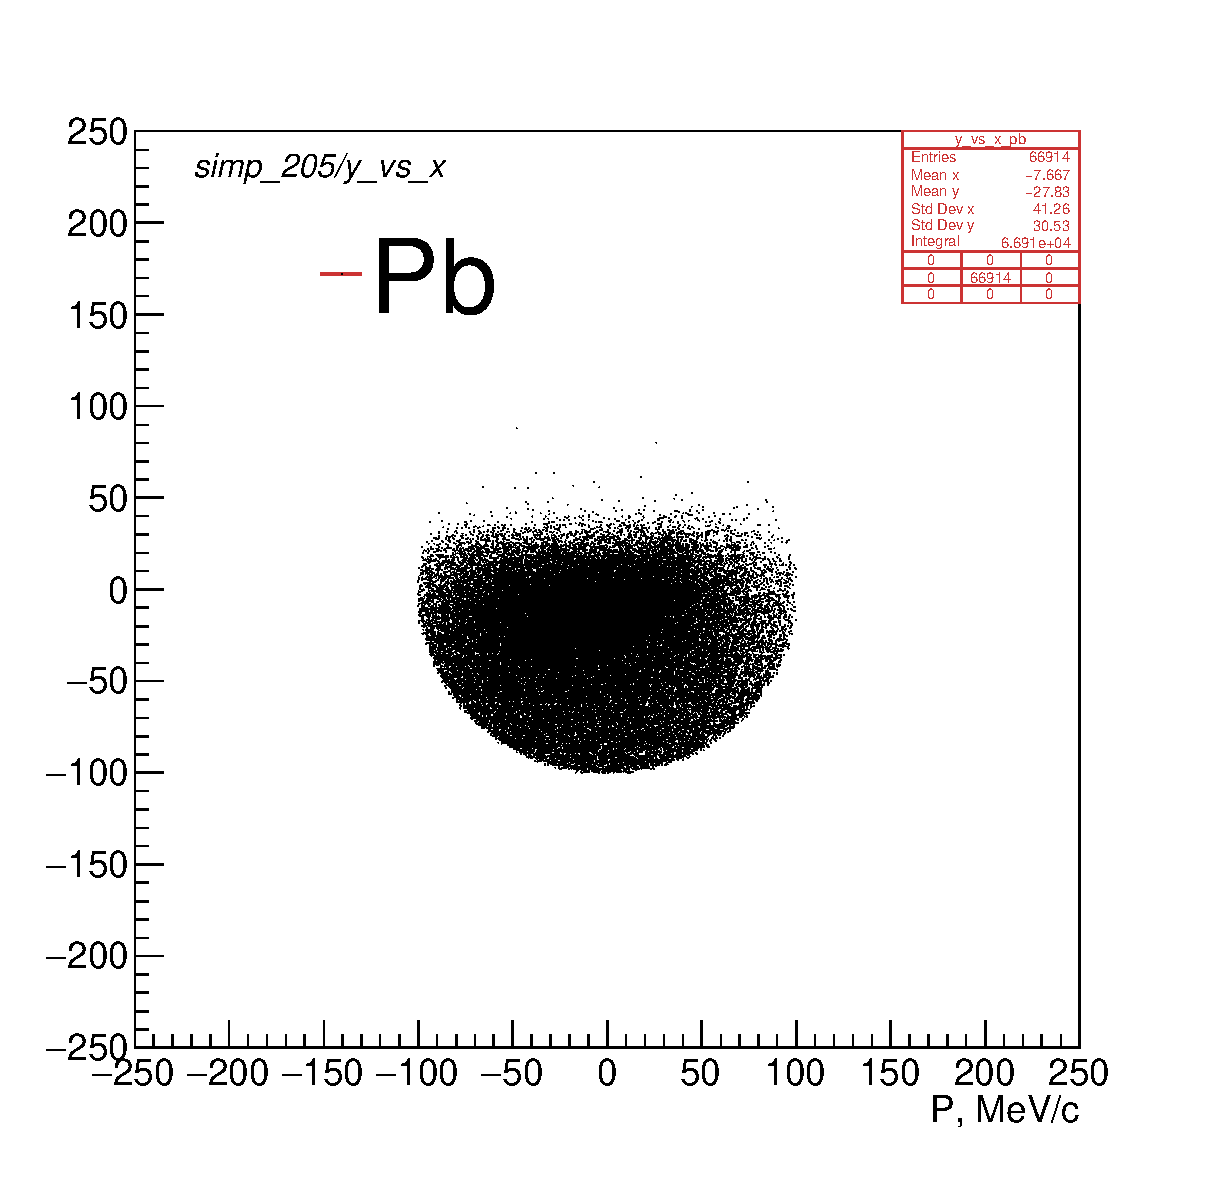
\includegraphics[width=0.5\textwidth]{png/figure_00035}
      %}
    };
    \node[anchor=south west,inner sep=0] at (0,-10.) {
      % \node[shift={(0 cm,0.cm)},inner sep=0,rotate={90}] at (0,0) {}
      % \makebox[\textwidth][c] {
        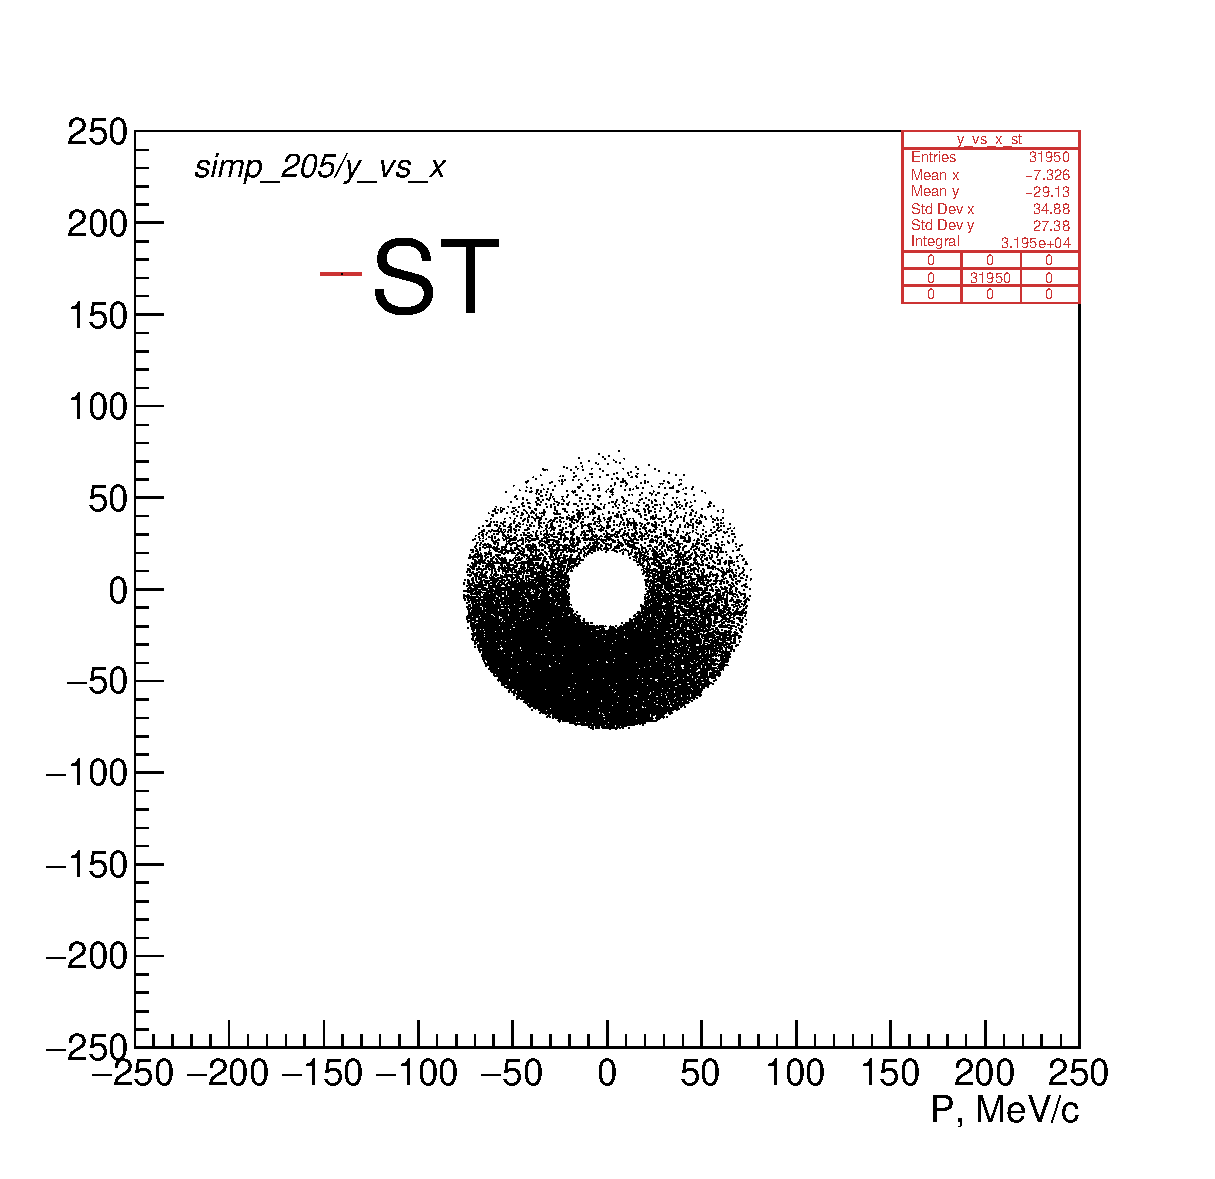
\includegraphics[width=0.5\textwidth]{png/figure_00031}
      % }
    };
    % \node [text width=8cm, scale=1.0] at (14.5,0.5) {$\mu_B$, expected background mean};
    % \node [text width=8cm, scale=1.0, rotate={90}] at (1.5,7.5) { $S_{D}$, ``discovery'' signal strength  };
  \end{tikzpicture}
  \caption{
    \label{figure:y_vs_x_st}
    Y(stop):X(stop) for pions stopped in the CH2, Pb, and ST
  }
\end{figure}


%%% Local Variables:
%%% mode: latex
%%% TeX-master: t
%%% End:

\section{Reconstructed photon spectrum}

For the photon energy of $\sim$ 130 MeV, the present reconstruction code is not expected
to reconstruct $\gamma \to e^+e^-$ events efficiently.

{\red run reconstruction and demonstrate that ? }

However, the intrinsic resolution of the tracker should contribute less than 0.5 MeV to the
reconstructed full width of the $e^+e^-$ conversion peak.

We therefore use the MC truth - the sum of the two MC particle momenta recorded in front
of the tracker - as a proxy to the reconstructed photon momentum
%%%%%%%%%%%%%%%%%%%%%%%%%%%%%%%%%%%%%%%%%%%%%%%%%%%%%%%%%%%%%%%%%%%%%%%%%%%%%%
\subsection{Contribution of the $\rm CH_2$ disk }
\begin{itemize}
\item
  compare 1mm to 0.1 mm to 0.2mm
\end{itemize}

%%%%%%%%%%%%%%%%%%%%%%%%%%%%%%%%%%%%%%%%%%%%%%%%%%%%%%%%%%%%%%%%%%%%%%%%%%%%%%
\subsection{Contribution of the Pb foil}

Spectrum has been measured in \cite{RPC_1977_Baer}
\begin{itemize}
\item
  compare 1mm to 0.1 mm to 0.2mm
\end{itemize}


%%% Local Variables:
%%% mode: latex
%%% TeX-master: t
%%% End:

%
\section{Status of the track reconstruction}

%%% Local Variables:
%%% mode: latex
%%% TeX-master: t
%%% End:

%
\section{Option 2: converter inside the OPA}
\label{section:geometry_v4}
If the converter radius is large enough, the converter ring surrounding the pion degrader
could be limiting the degrader arm movement. 
An attractive option of positioning the converter is to have the converter placed 
at the upstream end of the OPA. In this case, a gold converter foil could be put
on a thin ring made of fiber foam and supported by the OPA, similar to the stopping target.
That would allow to make a converter ring wider and increase the yield of $\gamma \to e^+e^-$
events and simplify geometry of the moving part of the degrader positioned inside
a narrow gap in between the TS and OPA.

\begin{figure}[H]
  \begin{tikzpicture}
    \node[anchor=south west,inner sep=0] at (0,0.) {
      % \node[shift={(0 cm,0.cm)},inner sep=0,rotate={90}] at (0,0) {}
      \makebox[\textwidth][c] {
        \includegraphics[width=0.90\textwidth]{png/pipenu_cele3b0_geom_degrader}
      }
    };
    % \node [text width=8cm, scale=1.0] at (14.5,0.5) {$\mu_B$, expected background mean};
    % \node [text width=8cm, scale=1.0, rotate={90}] at (1.5,7.5) { $S_{D}$, ``discovery'' signal strength  };
  \end{tikzpicture}
  \caption{
    \label{figure:degrader_v4}
    degrader v4: converter ring supported by OPA
  }
\end{figure}

%%%%%%%%%%%%%%%%%%%%%%%%%%%%%%%%%%%%%%%%%%%%%%%%%%%%%%%%%%%%%%%%%%%%%%%%%%%%%%
\subsection{Parameters used in the simulation}

\begin{itemize}
\item
  pion stops: reuse pipenu:bpim01b0, for the next iteration resimulate properly
\item
  converter thickness - 100$\mu$, width - 2 cm, $R_{out} = 250$ mm
\item 
  for simulating RPC photons: degrader material: CH2 , 24mm thick,
  to approximately match the material of 4mm thick Ti converter.
  May need to re-optimize the thickness to match the pion stopping rate
  at the ST to that of 4mm Ti
\item
  10M events $\gamma$ events, 
\item
  simulated range of cos(theta): [0,0.45] 
\item
  dataset family: rpc07b0
\end{itemize}

%%%%%%%%%%%%%%%%%%%%%%%%%%%%%%%%%%%%%%%%%%%%%%%%%%%%%%%%%%%%%%%%%%%%%%%%%%%%%%
\subsection{Resolution in the photon energy}

The distribution of $E_\gamma = P(e^+) + P(e^-)$ for the events with the reconstructed
$e^+$ and $e^-$ tracks is shown in Figure~\ref{figure:t2_0_smom_1}.
Overlaid is the fit of the distribution with the SU2020 function \cite{SU2020}.
The $\chi^2/DOF$ of the fit is close to one, and with about 1000 events in the peak,
an uncertainty on the peak position returned by the fitter is below 10 keV/c.
This is a good indication that statistics of 1000 events should be sufficient
to achieve the momentum scale calibration accuracy of 100 keV/c.

\begin{figure}[H]
  \begin{tikzpicture}
    \node[anchor=south west,inner sep=0] at (0,0.) {
      % \node[shift={(0 cm,0.cm)},inner sep=0,rotate={90}] at (0,0) {}
      \makebox[\textwidth][c] {
        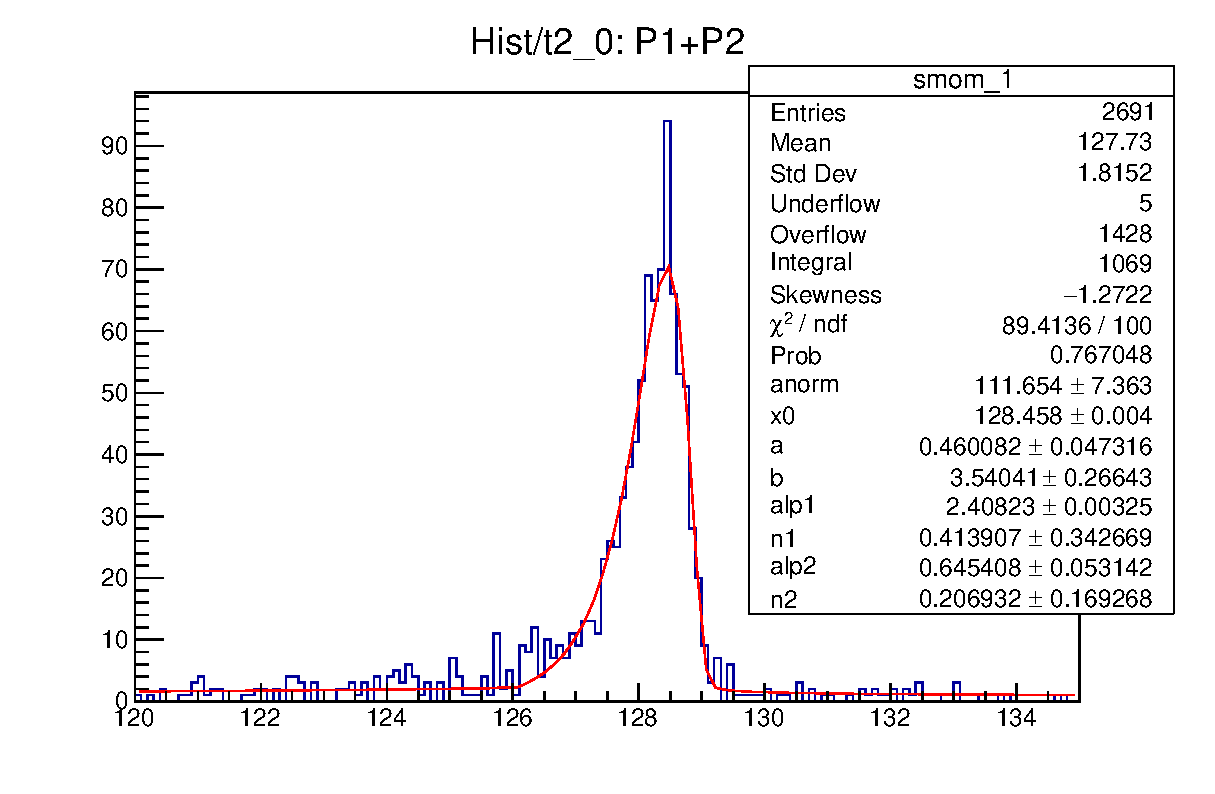
\includegraphics[width=0.95\textwidth]{pdf/figure_00082}
      }
    };
    % \node [text width=8cm, scale=1.0] at (14.5,0.5) {$\mu_B$, expected background mean};
    % \node [text width=8cm, scale=1.0, rotate={90}] at (1.5,7.5) { $S_{D}$, ``discovery'' signal strength  };
  \end{tikzpicture}
  \caption{
    \label{figure:t2_0_smom_1}
    Distribution of $E_\gamma = P(e^+) + P(e^-)$ for events with two reconstructed tracks
  }
\end{figure}

%%%%%%%%%%%%%%%%%%%%%%%%%%%%%%%%%%%%%%%%%%%%%%%%%%%%%%%%%%%%%%%%%%%%%%%%%%%%%%
\newpage
\subsection{Converter impact on the CE acceptance}

Figure~\ref{figure:ce_momentum_tsda} compares acceptances for the reconstructed CE tracks
got default geometry and geometry w/o the converter.
\begin{itemize}
\item 
  CE on Al for this comparison have been generated with the radiative corrections
  taken into account in the LL approximation.
\item 
  A model of perfect detector has been used - no misalignments, no miscalibrations.
\item
  2.5M events simulated per configuration.
\end{itemize}

Plotted in Figure~\ref{figure:ce_acceptance} are the momentum distributions for all
reconstructed CE tracks, w/o any selections applied. 

Comparison of the distributions tells that for the momentum window of [103,105] MeV/c,
an introduction of the Au converter reduces the CE acceptance by 0.16\%.

\begin{figure}[H]
  \begin{tikzpicture}
    \node[anchor=south west,inner sep=0] at (0,0.) {
      % \node[shift={(0 cm,0.cm)},inner sep=0,rotate={90}] at (0,0) {}
      % \makebox[\textwidth][c] {
        \includegraphics[width=0.54\textwidth]{pdf/figure_00051}
      % }
    };
    \node[anchor=south west,inner sep=0] at (9.8,0.) {
      % \node[shift={(0 cm,0.cm)},inner sep=0,rotate={90}] at (0,0) {}
      % \makebox[\textwidth][c] {
        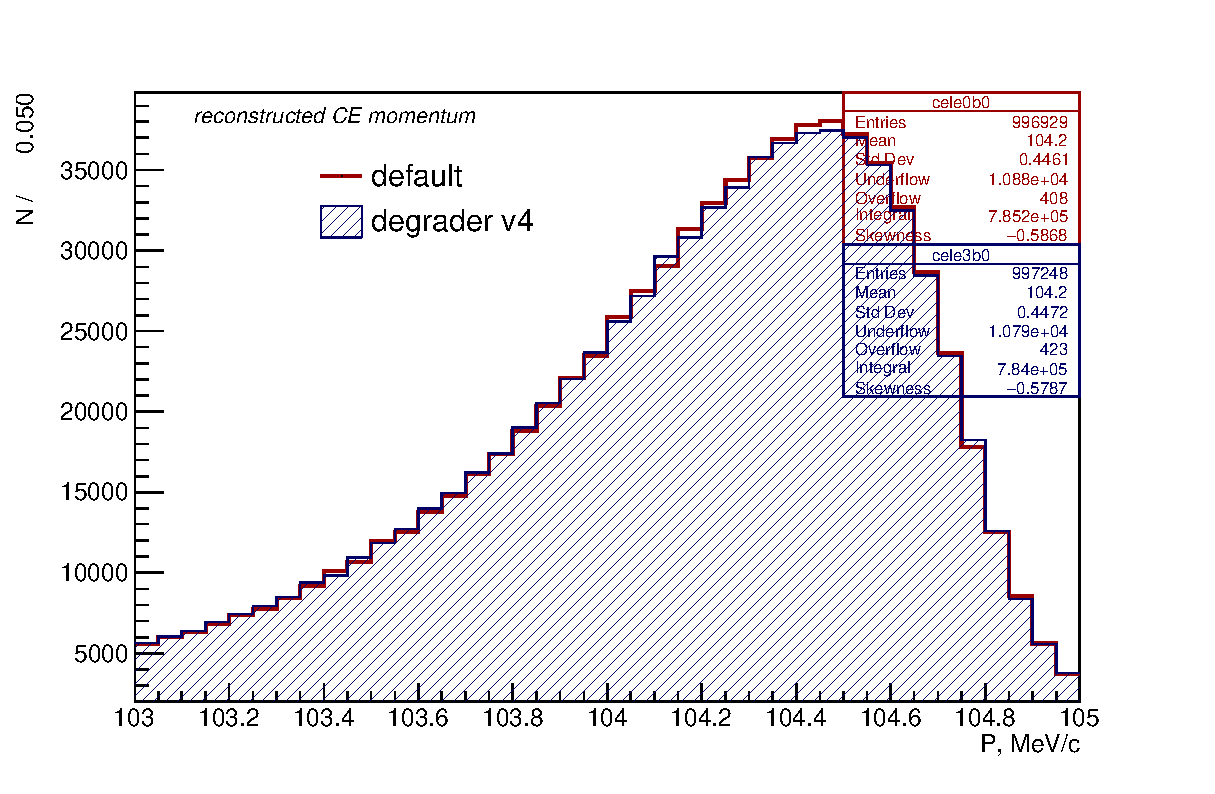
\includegraphics[width=0.54\textwidth]{pdf/figure_00052}
      % }
    };
    % \node [text width=8cm, scale=1.0] at (14.5,0.5) {$\mu_B$, expected background mean};
    % \node [text width=8cm, scale=1.0, rotate={90}] at (1.5,7.5) { $S_{D}$, ``discovery'' signal strength  };
  \end{tikzpicture}
  \caption{
    \label{figure:ce_acceptance}
    CE momentum distribution for two geometries, with and without the converter ring. 
  }
  \label{figure:ce_momentum_tsda}
\end{figure}
%%% Local Variables:
%%% mode: latex
%%% TeX-master: t
%%% End:

% %
\section{Impact on the CE acceptance}

\begin{itemize}
\item
  two geometry options: default vs 'converter in'
\item
  for each option: 2.5 CE events, LO, perfect geometry
\end{itemize}

Distributions in Figure~\ref{figure:ce_momentum} show an impact of a 2cm wide, 100 um thin
gold converter ring on the CE acceptance. Shown there are the reconstructed CE momentum
distributions for two geometries - 'default' vs 'default plus converter ring'.

Plotted are all reconstructed tracks, no selections.

Within statistical uncertainties, the total number of the reconstructed tracks doesn't change.

Adding the converter ring reduces the number of tracks in the momentum range 103.0-105.0 MeV/c
by $\sim$ 0.2\%.

\begin{figure}[H]
  \begin{tikzpicture}
    \node[anchor=south west,inner sep=0] at (0,0.) {
      % \node[shift={(0 cm,0.cm)},inner sep=0,rotate={90}] at (0,0) {}
      % \makebox[\textwidth][c] {
        \includegraphics[width=0.54\textwidth]{pdf/figure_00051}
      % }
    };
    \node[anchor=south west,inner sep=0] at (9.8,0.) {
      % \node[shift={(0 cm,0.cm)},inner sep=0,rotate={90}] at (0,0) {}
      % \makebox[\textwidth][c] {
        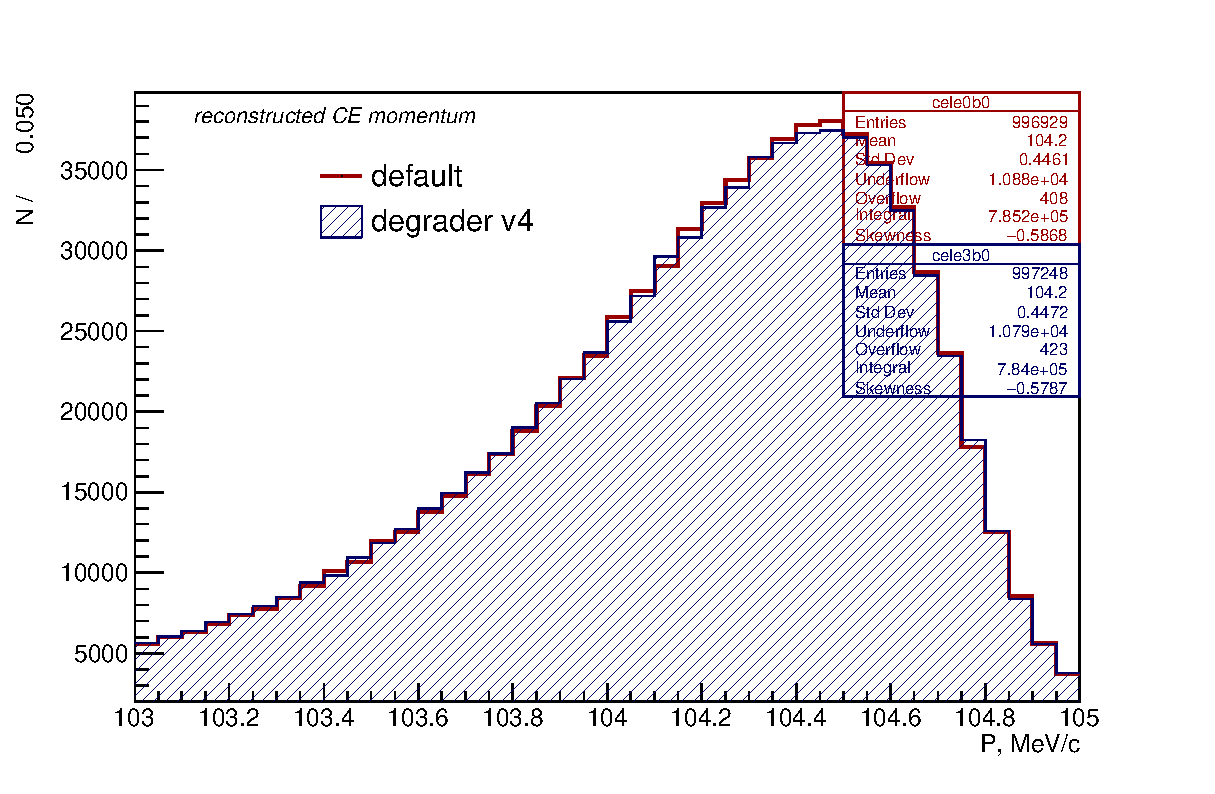
\includegraphics[width=0.54\textwidth]{pdf/figure_00052}
      % }
    };
    % \node [text width=8cm, scale=1.0] at (14.5,0.5) {$\mu_B$, expected background mean};
    % \node [text width=8cm, scale=1.0, rotate={90}] at (1.5,7.5) { $S_{D}$, ``discovery'' signal strength  };
  \end{tikzpicture}
  \caption{
    \label{figure:ce_acceptance}
    CE momentum distribution for two geometries, with an without the converter ring
  }
  \label{figure:ce_momentum}
\end{figure}


%%% Local Variables:
%%% mode: latex
%%% TeX-master: t
%%% End:
 % included into geometry_v4

%%%%%%%%%%%%%%%%%%%%%%%%%%%%%%%%%%%%%%%%%%%%%%%%%%%%%%%%%%%%%%%%%%%%%%%%%%%%%%
\section{Electric current}
When inserted into the beam, the degrader stops the beam particles, which are
mostly low energy, MeV-range, electrons. To avoid the accumulation of the electric charge,
the degrader needs to be grounded. An estimate of the electric current can be obtained
as follows:
\begin{itemize}
\item
  assume that degrader stops all beam flash particles
\item
  from SU2020: the rate of the beam flash particles, assume all are electrons, is $\sim ~ 10^2$ of that of muons
\item
  muons : $1.6 \cdot 10^{-3} \times 3.9 \cdot 10^7$ , say, $7 \cdot 10^4$, which gives $\sim ~ 7 \cdot 10^7$ electrons per 1.7 ms
\item
  the corresponding electric current is $I ~=~ 7 \cdot 10^{-7} \times 1.6 \cdot 10^{-19} / {1.7 \cdot 10^{-6}} \sim 7 \cdot 10^{-6}$ A,
  or $\sim$ 10 microamperes
\end{itemize}

%%%%%%%%%%%%%%%%%%%%%%%%%%%%%%%%%%%%%%%%%%%%%%%%%%%%%%%%%%%%%%%%%%%%%%%%%%%%%%
\section{Estimate of the time needed for momentum calibration}
Calibration with RPC on hydrogen allows to determine the momentum scale of the experiment.

In this section we assume that the experimental background doesn't affect
the determination accuracy of the momentum edge of RPC photon peak
and estimate the time needed for the calibration.

\kate{
\begin{itemize}
\item 
From $ 2.5 \times 10^8 $ protons on target, 67.42 negative pions stop on the $\rm{CH_2}$ part of the degrader at T>200ns.
\item 
A negative pion stopped in $\rm{CH_2}$ has a probability of about $ 5 \times 10^{-3} $ of producing a 129.4 MeV RPC photon from capture on hydrogen (Section 3).
\item 
The optimal geometry from Section 4 places a gold converter at radius R=25.0cm with thickness 0.1mm. Of $10^5$ RPC photons generated with angle 0<$\cos \theta$<0.1, 139 produce $e^+ e^-$ pairs that can likely be reconstructed in the tracker. Events counted as likely reconstructable have $e^+$ and $e^-$ each with at least 20 straw hits and momentum P > 30MeV/c. 
\end{itemize}
The product of these first three factors is a calibration event rate on the order of $10^{-12} $ per POT.
}

\begin{itemize}
\item 
  required accuracy of the momentum scale calibration $@$100 MeV/c: $\sigma_P/P$ < 100 keV/c
\item
  {\red how many events do we need ?} \kate{Estimates in the remaining items assume that 1000 $ \gamma \to e^+ e^- $ events would be sufficient to reconstruct the high-energy edge of the 129.4 MeV RPC photon momentum distribution.}
\item
  \kate{For a yield of $10^{-12}$ events/POT, collecting 1000 events requires $10^{15}$ protons on target.
  In one-batch mode, an average expected pulse intensity is $1.6 \times 10^7$, with one pulse every 1695ns for about 0.4s of each 1.4s Main Injector cycle. The resulting rate is $2.7 \times 10^{12}$ protons/sec. }
%\item
%  For a yield of $10^{-13}$ events/POT, collecting 1000 events requires $10^{16}$ protons on target.
%  In one-batch mode, an average expected pulse intensity is $1.6 \times 10^7$, and
%  an average  pulse rate of 1$.6 \times 10^5$ pulses/sec correspond to the rate of $2.5 \times 10^{12}$ protons/sec.
\item
  Assuming running at 10\% of nominal beam intensity and the data collection efficiency of 50\%,
  collecting 1000 reconstructable \kate{ $ \gamma \to e^+ e^- $ events would require on the order of
  $10^{15}/( 0.1 \cdot 0.5 \cdot  2.7 \times 10^{12}) \sim 10^4$ seconds, achievable in} one day of running.
%\item
%  Assuming running at 10\% of nominal beam intensity and the data collection efficiency of 50\%,
%  collecting 1000 reconstructable \piplusenu\ events would require
%  $10^{16}/(1.25 \times 10^{11}) \sim 10^5$ seconds, or about one day of running.
\item
  running at 10\% of the nominal beam intensity in one-batch mode and with the digitization starting
  at 200 ns corresponds to the total number of background hits per microbunch of about 200,
  so the pileup at T>300 ns should not be a problem.
\end{itemize}

\kate{
\bigskip
  Potential changes:
  \begin{itemize}
  \item 
    Update with simulation results using larger photon angle. Earlier results here follow Section 4 for consistency. 
  \end{itemize}
}
%%% Local Variables:
%%% mode: latex
%%% TeX-master: t
%%% End:


%%%%%%%%%%%%%%%%%%%%%%%%%%%%%%%%%%%%%%%%%%%%%%%%%%%%%%%%%%%%%%%%%%%%%%%%%%%%%% 
\section {Summary}

The pion degrader reduces the background from muon decays in flight to facilitate
the momentum scale calibration with \piplusenu\ decays. That calibration needs to
be performed at $B \simeq 0.7$ T, so the determined momentum scale would need to be
extrapolated to the nominal field value, B = 1 T.

With small modifications, the pion degrader could become an instrument
for calibrating the Mu2e momentum scale in full field. This calibration is based on
reconstruction of a 129.4 MeV photon peak in the $e^+e^-$ invariant mass spectrum.
%
This note demonstrates that due to small multiple scattering the sum of the
electron an positron momenta gives a good approximation of the $e^+e^-$ invariant mass.

Under realistic assumptions, the time needed to calibrate the momentum scale
to the accuracy better then 100 keV while running at 10\% of the nominal proton beam
intensity is about one day.


%%%%%%%%%%%%%%%%%%%%%%%%%%%%%%%%%%%%%%%%%%%%%%%%%%%%%%%%%%%%%%%%%%%%%%%%%%%%%%
%
%%%%%%%%%%%%%%%%%%%%%%%%%%%%%%%%%%%%%%%%%%%%%%%%%%%%%%%%%%%%%%%%%%%%%%%%%%%%%%
\newpage
\bibliographystyle{unsrtnat}
\bibliography{clfv,mu2e_internal_notes,mu2e_piplusenu_notes,radiative_pion_capture}

% \include{appendix_a}
\appendix

%%%%%%%%%%%%%%%%%%%%%%%%%%%%%%%%%%%%%%%%%%%%%%%%%%%%%%%%%%%%%%%%%%%%%%%%%%%%%%
\section {Datasets}
\label{appendix_b}

\begin{itemize}
\item 
  Definition of the datasets used for this study and the book-keeping information
  can be found at \\
  \href{https://github.com/sridhar130/pipenu/blob/main/doc/datasets.org}
  {\blue https://github.com/sridhar130/pipenu/blob/main/doc/datasets.org}.
\item
  the datasets and stntuples are available from {\bf mu2egpvm*:/exp/mu2e/data/projects/pipenu}
\item
  location of the stntuple catalogs : \\
  \href{https://mu2e.fnal.gov/public/hep/computing/Stntuple/cafdfc/pipenu/index.shtml}
  {\blue https://mu2e.fnal.gov/public/hep/computing/Stntuple/cafdfc/pipenu/index.shtml}
\end{itemize}

%%% Local Variables:
%%% mode: latex
%%% TeX-master: t
%%% End:


\end{document}
